\documentclass[tikz,border=8pt]{standalone}
% Shared look for every TikZ diagram. Load with \input{../../tools/tikz-style.tex}
\usepackage[T1]{fontenc}
\usepackage{lmodern}
\renewcommand{\sfdefault}{lmr}  % diagrams use the same serif as the text
\usetikzlibrary{arrows.meta, positioning, shapes.geometric, calc, fit, backgrounds}
\definecolor{cblue}{HTML}{4C78A8}
\definecolor{corange}{HTML}{F58518}
\definecolor{cgreen}{HTML}{54A24B}
\definecolor{cred}{HTML}{E45756}
\definecolor{cpurple}{HTML}{B279A2}
\definecolor{cgrey}{HTML}{6B6B6B}
\tikzset{
  every picture/.style={font=\sffamily, line width=1.2pt},
  box/.style={draw=#1, fill=#1!12, rounded corners=4pt, align=center, inner sep=7pt, minimum height=1.1cm},
  box/.default=cgrey,
  arrow/.style={-{Stealth[length=3mm]}, draw=cgrey, line width=1.4pt},
  title/.style={font=\sffamily\bfseries\Large},
  note/.style={font=\sffamily\small, text=cgrey, align=center},
}
\AtBeginDocument{\hyphenpenalty=10000 \exhyphenpenalty=10000}

\begin{document}
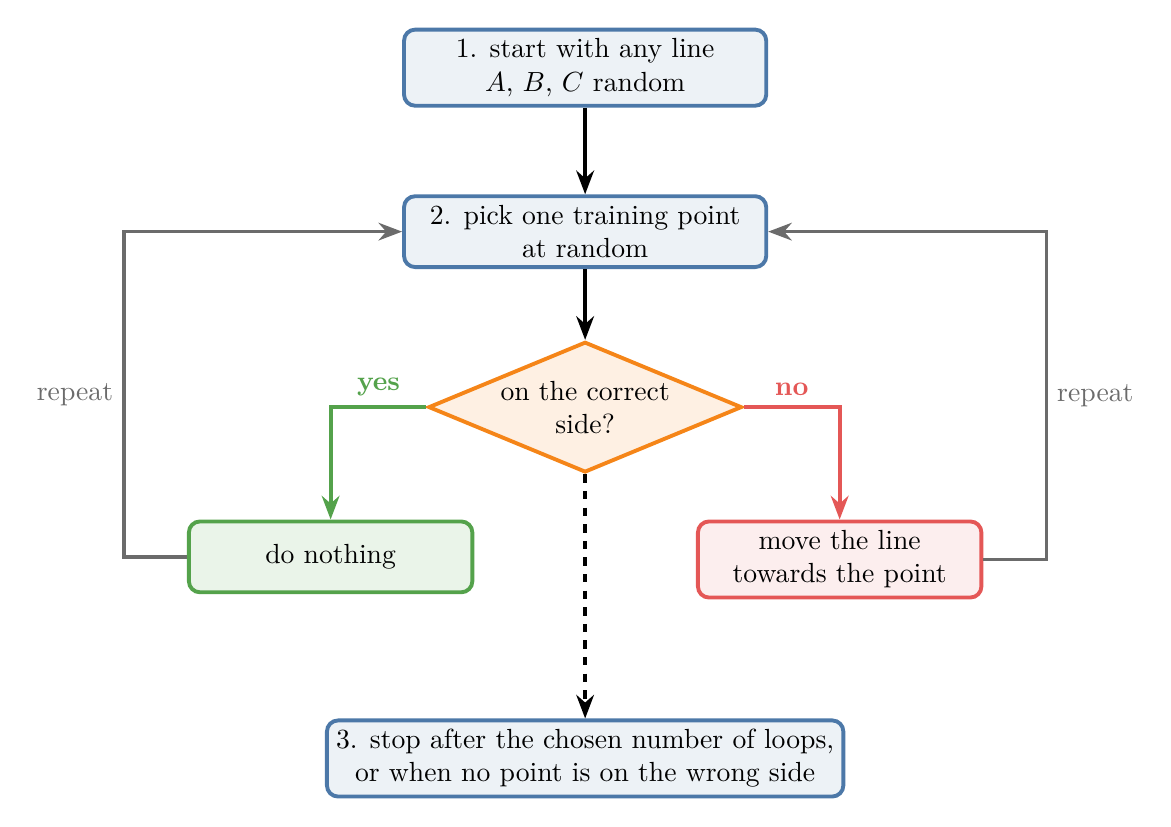
\begin{tikzpicture}[node distance=1.1cm,
  box/.style={rounded corners=4pt, draw=cblue, fill=cblue!10, line width=1.4pt, minimum width=4.6cm, minimum height=0.9cm, align=center},
  ask/.style={diamond, aspect=2.4, draw=corange, fill=corange!12, line width=1.4pt, inner sep=1pt, align=center},
  good/.style={rounded corners=4pt, draw=cgreen, fill=cgreen!12, line width=1.4pt, minimum width=3.6cm, minimum height=0.9cm, align=center},
  bad/.style={rounded corners=4pt, draw=cred, fill=cred!10, line width=1.4pt, minimum width=3.6cm, minimum height=0.9cm, align=center}]
  \node[box] (start) {1. start with any line\\$A$, $B$, $C$ random};
  \node[box, below=of start] (pick) {2. pick one training point\\at random};
  \node[ask, below=0.9cm of pick] (q) {on the correct\\side?};
  \node[good, below left=1.0cm and 0.4cm of q] (yes) {do nothing};
  \node[bad, below right=1.0cm and 0.4cm of q] (no) {move the line\\towards the point};
  \node[box, below=3.1cm of q] (stop) {3. stop after the chosen number of loops,\\or when no point is on the wrong side};
  \draw[-{Stealth[length=3mm]}, line width=1.4pt] (start) -- (pick);
  \draw[-{Stealth[length=3mm]}, line width=1.4pt] (pick) -- (q);
  \draw[-{Stealth[length=3mm]}, line width=1.4pt, cgreen] (q) -| node[pos=0.25, above, font=\bfseries] {yes} (yes);
  \draw[-{Stealth[length=3mm]}, line width=1.4pt, cred] (q) -| node[pos=0.25, above, font=\bfseries] {no} (no);
  \draw[-{Stealth[length=3mm]}, line width=1.2pt, cgrey] (yes.west) -- ++(-0.8,0) |- node[pos=0.25, left] {repeat} (pick.west);
  \draw[-{Stealth[length=3mm]}, line width=1.2pt, cgrey] (no.east) -- ++(0.8,0) |- node[pos=0.25, right] {repeat} (pick.east);
  \draw[-{Stealth[length=3mm]}, line width=1.2pt, dashed] (q.south) -- (stop.north);
\end{tikzpicture}
\end{document}
